\subsection{Wdrożenie Lupus}

Sekcja opisuje użycie Lupus jako \textbf{Systemu Sterowania} dla \textbf{Problemu Zarządzania} opisanego w następnej podsekcji dla emulatora sieci 5G, który przyjmie z kolei rolę \textbf{Systemu Zarządzanego}. 

\subsubsection{Problem Zarządzania}

Celem jest utrzymanie żądanych wartości zasobów dla funkcji płaszczyzny użytkownika (ang. \textit{User Plane Function, UPF}) na optymalnym poziomie. Optymalność oznacza zapewnienie wystarczających zasobów do obsługi obciążenia, ale jednocześnie unikanie ich nadmiernego przydziału, co pozwala na ograniczenie niepotrzebnych kosztów związanych z wynajmem zasobów chmurowych.

W ramach wdrożenia Open5GS, w tym dla komponentu UPF, istnieje kilka instancji uruchomieniowych (ang. \textit{Deployments}) jak pokazano na rysunku \ref{fig:53-depy}.


\begin{figure}[!h]
    \centering 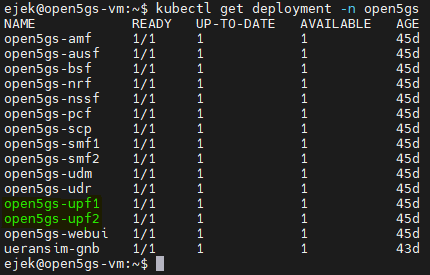
\includegraphics[width=1\linewidth]{53-depy.png}
    \caption{Wdrożenia Open5GS, w tym instancje UPF}\label{fig:53-depy}
\end{figure}

Każdy \textit{pod} w klastrze Kubernetes posiada zdefiniowane wartości dotyczące przydziału zasobów:

\begin{itemize}
    \item \textbf{\texttt{requests}} – określa ilość zasobów CPU oraz pamięci operacyjnej (RAM), jaką dany pod żąda od środowiska chmurowego. Kubernetes zapewnia, że węzeł posiada wystarczające zasoby, aby spełnić te wymagania przed przydzieleniem poda do \textit{węzła}.
    \item \textbf{\texttt{limits}} – maksymalna ilość zasobów, jaką pod może zużyć. Przekroczenie tych wartości skutkuje zakończeniem procesu (np. jego ubiciem w celu ochrony środowiska).
\end{itemize}

Dodatkowo możliwe jest monitorowanie rzeczywistego (aktualnego, chwilowego) wykorzystania procesora i pamięci operacyjnej.

\textbf{Mechanizmy dostępne w Kubernetes}

Kubernetes umożliwia:
\begin{itemize}
    \item monitorowanie bieżącego zużycia CPU oraz pamięci dla konkretnego poda,
    \item monitorowanie zdefiniowanych wartości \texttt{requests} i \texttt{limits} dla konkretnego poda,
    \item aktualizację wartości \texttt{requests} i \texttt{limits} dla konkretnego poda.
\end{itemize}

Wdrożenie komponentu UPF w repozytorium \href{https://github.com/niloysh/open5gs-k8s}{open5gs-k8s} wykorzystuje następujące wartości zasobów:

\begin{lstlisting}[language=sh, caption=Konfiguracja zasobów dla UPF w Open5GS]
resources:
  requests:
    memory: "256Mi"
    cpu: "200m"
  limits:
    memory: "512Mi"
    cpu: "500m"
\end{lstlisting}

Niniejsza konfiguracja jest traktowana jako \textbf{punkt operacyjny}, który powinien być wystarczający w normalnych warunkach (np. przez 80\% czasu). Jednak w sytuacjach, gdy pojedynczy pod UPF sporadycznie przekracza te wartości, konieczne jest zwiększenie dostępnych zasobów oraz proporcjonalne podniesienie limitów.

Zakłada się, że każdorazowe przekroczenie wartości operacyjnych CPU lub pamięci skutkuje przydzieleniem dodatkowych 20\% zasobów dla \texttt{requests} oraz ustawieniem \texttt{limits} na poziomie dwukrotności nowej wartości \texttt{requests}.

\textbf{Przykładowa adaptacja zasobów}

\begin{itemize}
    \item Gdy zużycie CPU osiąga wartość \texttt{270m}:
    \begin{itemize}
        \item \texttt{requests} zostaje zwiększone do \( 270m \times 1.2 = 324m \),
        \item \texttt{limits} zostaje zwiększone do \( 324m \times 2 = 648m \).
    \end{itemize}
    \item Analogiczne zasady dotyczą przydziału pamięci operacyjnej.
\end{itemize}

Jeśli rzeczywiste wykorzystanie zasobów jest znacząco niższe od wartości operacyjnej, nie jest podejmowana żadna akcja korygująca. Nadmierne skalowanie w dół skutkowałoby zbyt częstymi restartami podów, co w konsekwencji generowałoby większe koszty niż wynikające z niedostatecznego wykorzystania zasobów.

\subsubsection{Implementacja Agentów Translacji}

\textbf{Agent Ingress}

Agent Ingress okresowo pobiera aktualne zużycie zasobów oraz zdefiniowane wartość \texttt{requests} oraz \texttt{limits} dla podów UPF w obu wdrożeniach (ang. \textins{deployments}). Następnie zgodnie ze specyfikacją interfejsu \textbf{Lupin} będzie aktualizował pole \texttt{Input} statusu obiektu API \textbf{Elementu Ingress} obiektem JSON jak pokazano na listingu \ref{lst:521} z przykładowymi wartościami. Jednocześnie takowy obiekt JSON będzie stanowił początkową postać \textbf{danych}.

\begin{lstlisting}[language=sh, caption={\emph{}}\label{lst:521}]
    {
        "open5gs-upf1: {
            "actual": {
                "cpu": "1m",
                "memory": "18Mi"
            },
            "requests": {
                "cpu": "100m",
                "memory": "128Mi"
            },
            "limits": {
                "cpu": "250m",
                "memory": "256Mi"
            }
        },
        "open5gs-upf2: {
            "actual": {
                "cpu": "1m",
                "memory": "25Mi"
            },
            "requests": {
                "cpu": "200m",
                "memory": "256Mi"
            },
            "limits": {
                "cpu": "500m",
                "memory": "512Mi"
            }
        }
    }
\end{lstlisting}

Kod agenta Ingress znajduje się w załączniku //TODO.

\textbf{Agent Egress}

Agent Egress udostępnia endpoint HTTP, który przyjmuje dane w postaci przedstawionej na rysunku \ref{fig:53-egress}

\begin{figure}[!h]
    \centering 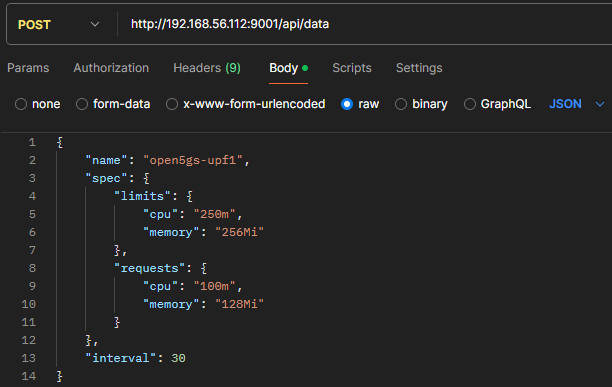
\includegraphics[width=1\linewidth]{53-egress.png}
    \caption{Endpoint Egress Agent przyjmujący finalne dane}\label{fig:53-egress}
\end{figure}

Następnie dla wdrożenia (ang. \textit{deployment}) zadanego polem \texttt{name} zmodyfikuje zdefiniowane wartości \texttt{requests} oraz \texttt{limits} według pola \texttt{spec}. Opcjonalne jest pole \texttt{interval}, które określa z jakim interwałem czasowym (w sekundach) raportować aktualne zużycie zasobów. Agent Egress odpowiednio wysteruje tym polem Agenta Ingress.

\subsubsection{Planowanie Logiki Pętli}

Analizując dane wejściowe z listingu \ref{lst:521} można wyróżnić cztery możliwe stany pojedynczego wdrożenia UPF:
\begin{itemize}
    \item \textbf{NORMAL} – wartości \texttt{requests} i \texttt{limits} ustawione na wartości domyślne, rzeczywiste zużycie (\texttt{actual}) pozostaje poniżej wartości domyślnych.
    \item \textbf{NORMAL\_TO\_CRITICAL} – wartości \texttt{requests} i \texttt{limits} nadal są domyślne, ale rzeczywiste zużycie (\texttt{actual}) przekracza wartości domyślne.
    \item \textbf{CRITICAL} – wartości \texttt{requests} i \texttt{limits} przekraczają wartości domyślne, a rzeczywiste zużycie (\texttt{actual}) również pozostaje powyżej wartości domyślnych.
    \item \textbf{CRITICAL\_TO\_NORMAL} – wartości \texttt{requests} i \texttt{limits} nadal przekraczają wartości domyślne, ale rzeczywiste zużycie (\texttt{actual}) spadło poniżej wartości domyślnych.
\end{itemize}

W zależności od stanu systemu należy podjąć następujące działania:
\begin{itemize}
    \item \textbf{NORMAL} – brak działań, system działa poprawnie.
    \item \textbf{NORMAL\_TO\_CRITICAL} – dostosowanie wartości \texttt{requests} i \texttt{limits}, ustawienie interwału obserwacji na wysoki (\texttt{HIGH}).
    \item \textbf{CRITICAL} – dostosowanie wartości \texttt{requests} i \texttt{limits} do aktualnego zapotrzebowania.
    \item \textbf{CRITICAL\_TO\_NORMAL} – przywrócenie wartości \texttt{requests} i \texttt{limits} do wartości domyślnych, ustawienie interwału obserwacji na niski (\texttt{LOW}).
\end{itemize}

W związku z powyższym opisem pętla powinna w każdej iteracji określi punkt pracy, czyli stan w jakim znajduje się UPF. Jeśli jest to stan \texttt{NORMAL}, nie ma potrzeby aby wykonywać jakiekolwiek akcje sterujące. W przeciwnym wypadku, należy "dostroić" UPF odpowiednimi wartościami \texttt{requests} oraz \texttt{limits}. Jeśli UPF jest lub zbliża się do stanu krytycznego należy je ustawić z odpowiednim zapasem, zaś jeżeli UPF wraca już do stanu normalnego należ przywrócić im wartości domyślne. Na sam koniec, jeżeli mamy jeden ze stanów przejściowych (\texttt{NORMAL\_TO\_CRITICAL} bądź \texttt{CRITICAL\_TO\_NORMAL}) należy zmienić interwał obserwacji odpowiednio na wysoki lub niski.

Z tego opisu widzimy, że \textbf{Część obliczeniowa} logiki pętli składa się z trzech części:
\begin{itemize}
    \item Ustalenie punktu pracy 
    \item Obliczenie wartości \texttt{requests} oraz \texttt{limits}
    \item Ustalenie wartości interwału na podstawie punkty pracy
\end{itemize}

Dlatego też powstaną trzy \textbf{Elementy Zewnętrzne}:
\begin{itemize}
    \item \textbf{POINT} – akceptuje \texttt{"*"} (wszystkie pola danych), zwraca \texttt{"point"}.
    \item \textbf{SPEC} – akceptuje \texttt{"actual"}, zwraca \texttt{"spec"} zawierające wartości \texttt{"requests"} oraz \texttt{"limits"}.
    \item \textbf{INTERVAL} – akceptuje \texttt{"point"}, zwraca \texttt{"interval"}.
\end{itemize}

A \textbf{Workflow Akcji} dla \textbf{Elementu Lupus} odpowiedzialnego za rekoncylację jednego wdrożenia będzie wyglądało jak na rysunku \ref{fig:53-workflow-akcji}

\begin{figure}[!h]
    \centering 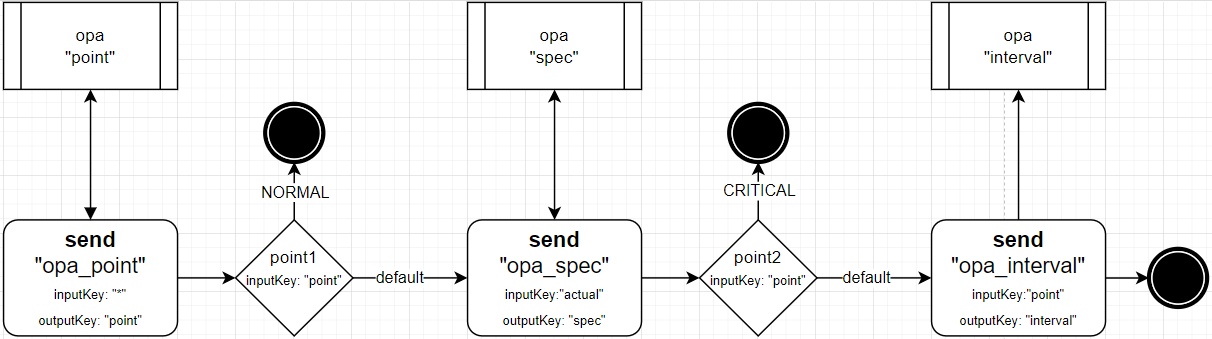
\includegraphics[width=1\linewidth]{53-workflow-akcji.png}
    \caption{Workflow Akcji Elementu Lupus}\label{fig:53-workflow-akcji}
\end{figure}

\subsubsection{Przygotowanie Elementów Zewnętrznych}

Każdy z elementów zewnętrznych przygotowano jako aplikacje python emulujące serwer Open Policy Agent.

Implementacje można znaleźć w załączniku //TODO.

\subsubsection{Wyrażenie workflow pętli w notacji LupN}

\textbf{Workflow Pętli} pokazano na rysunku \ref{fig:53-workflow-petli}

\begin{figure}[!h]
    \centering 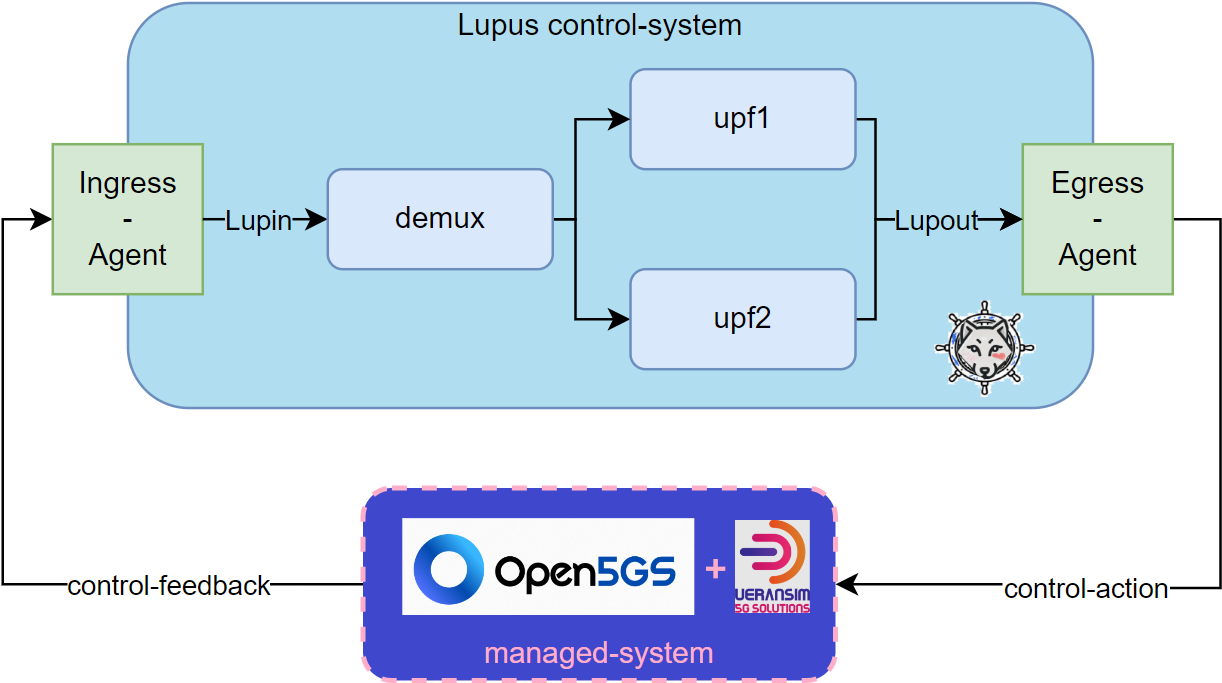
\includegraphics[width=1\linewidth]{53-workflow-petli.png}
    \caption{Workflow Pętli}\label{fig:53-workflow-petli}
\end{figure}

Element "demux" służy do rozdzielenia \textbf{danych} na dwie części. Każde wdrożenie UPF ma swój dedykowany element "upf1" lub "upf2", który obsługuje je według workflow akcji przedstawionej w poprzedniej podsekcji. Elementy "upf1" oraz "upf2" niezależnie pobudzają endpoint \texttt{/api/data} agenta egress.

Kod LupN znajduje się w załączniku //TODO. Ostatnim krokiem w celu uruchomienia pętli jest zaaplikowanie \textbf{pliku LupN}. 

\subsubsection{Prezentacja działania jednej iteracji pętli}
